\documentclass[usenames,dvipsnames,aspectratio=169]{beamer}

\usepackage[utf8]{inputenc}
\usepackage[T1]{fontenc}
\usepackage[magyar]{babel}
\usepackage{indentfirst}
\usepackage{listingsutf8}
\lstset{literate=
  {á}{{\'a}}1 {é}{{\'e}}1 {í}{{\'i}}1 {ó}{{\'o}}1 {ú}{{\'u}}1
  {Á}{{\'A}}1 {É}{{\'E}}1 {Í}{{\'I}}1 {Ó}{{\'O}}1 {Ú}{{\'U}}1
  {à}{{\`a}}1 {è}{{\`e}}1 {ì}{{\`i}}1 {ò}{{\`o}}1 {ù}{{\`u}}1
  {À}{{\`A}}1 {È}{{\'E}}1 {Ì}{{\`I}}1 {Ò}{{\`O}}1 {Ù}{{\`U}}1
  {ä}{{\"a}}1 {ë}{{\"e}}1 {ï}{{\"i}}1 {ö}{{\"o}}1 {ü}{{\"u}}1
  {Ä}{{\"A}}1 {Ë}{{\"E}}1 {Ï}{{\"I}}1 {Ö}{{\"O}}1 {Ü}{{\"U}}1
  {â}{{\^a}}1 {ê}{{\^e}}1 {î}{{\^i}}1 {ô}{{\^o}}1 {û}{{\^u}}1
  {Â}{{\^A}}1 {Ê}{{\^E}}1 {Î}{{\^I}}1 {Ô}{{\^O}}1 {Û}{{\^U}}1
  {œ}{{\oe}}1 {Œ}{{\OE}}1 {æ}{{\ae}}1 {Æ}{{\AE}}1 {ß}{{\ss}}1
  {ç}{{\c c}}1 {Ç}{{\c C}}1 {ø}{{\o}}1 {å}{{\r a}}1 {Å}{{\r A}}1
  {€}{{\EUR}}1 {£}{{\pounds}}1 {ő}{{\H{o}}}1
}
\lstdefinestyle{cpp}{
  language=[ISO]C++,
  showstringspaces=false,
  keywordstyle=\color{MidnightBlue}\bfseries,
  stringstyle=\color{DarkOrchid},
  commentstyle=\color{Brown},
  morecomment=[l][\color{OliveGreen}]{\#},
  breaklines=true,
  postbreak=\mbox{\textcolor{red}{$\hookrightarrow$}\space}
}
\usepackage{hyperref}
\usepackage{attachfile}
\usepackage{multirow}
% Navigációs pöttyök hozzáadása subsection nélküli fejezetekhez
\usepackage{remreset}
\makeatletter
\@removefromreset{subsection}{section}
\makeatother
\setcounter{subsection}{1}
%%%%%
\attachfilesetup{color={1.0 0.6 0.0},author={HFM},description={Kattintson duplán a minta %
megtekintéséhez!},icon=Paperclip}
\definecolor{kiemelesszin}{rgb}{0.6,0.0,0.0}
\definecolor{kiemelesszinZ}{rgb}{0.0,0.6,0.0}
\definecolor{kiemelesszinN}{RGB}{196,127,0}
\definecolor{hivatkozasszin}{rgb}{0.0,0.0,0.75}
\newcommand{\kiemel}[1]{{\color{kiemelesszin}#1}}
\newcommand{\kiemelZ}[1]{{\color{kiemelesszinZ}#1}}
\newcommand{\kiemelN}[1]{{\color{kiemelesszinN}#1}}
\newcommand{\hiv}[1]{{\color{hivatkozasszin}#1}}
\frenchspacing
\usetheme[compress]{Berlin}

\title[Modern szoftverfejlesztési eszközök - gMock]{gMock}
\subtitle{(GKxB\_INTM006)}
\author{Dr. Hatwagner F. Miklós}
\institute{Széchenyi István Egyetem, Győr}
\date{\hiv{\href{https://github.com/wajzy/GKxB\_INTM006.git}{https://github.com/wajzy/GKxB\_INTM006.git}}\\ \today}

\begin{document}

%1
\begin{frame}[plain]
    \titlepage
\end{frame}

\section{Bevezetés}

\begin{frame}
    \small
    Különféle tevékenységek céljai:
    \begin{description}[mm]
        \item[Egységtesztelés] \hfill\\ nyilvános interfészen elérhető szolgáltatások ellenőrzése bemenet-elvárt kimenet párokkal
        \item[Mockolás (kb. \emph{utánzás})] \hfill\\ objektumok közötti interfészek működésének ellenőrzése (gyakran még nem teljeskörűen implementált objektumokkal, ld. \hiv{\href{https://en.wikipedia.org/wiki/Test-driven_development}{TDD}}):
        \begin{itemize}
            \item Milyen metódusokat kell hívni?
            \item Milyen paraméterekkel?
            \item Mit kell visszaadniuk?
            \item Milyen sorrendben?
            \item Hányszor?
        \end{itemize}
      \end{description}
\end{frame}

\begin{frame}
    Tesztelési célból egy valódi objektumot helyettesítő objektum (test double) lehet:
    \begin{description}[m]
        \footnotesize
        \item[Dummy] \hfill \\ Soha nem használt objektum, jellemzően csak azért hozzák létre, hogy pl. egy metódusnak formálisan átadhassák. Pl. üres \texttt{Person} osztály.
        \item [Stub] \hfill \\ Előre bekészített válaszokat ad a tesztek során feltett kérdésekre, másra nem képes. Pl. a \texttt{Person} osztály példányai mindig ugyanazt a vezetéknevet adják vissza.
        \item [Spy] \hfill \\ Olyan \emph{stub}, ami rögzíti a hívás módját, mennyiségét. Pl. olyan osztály, ami rögzíti, melyik metódusát hányszor hívták.
        \item [Mock] \hfill \\ A hívásokkal kapcsolatban beprogramozott, specifikáció szerinti elvárásokat támaszt (pl. mennyiség, paraméterezés, sorrend), valamennyi tervezett szolgáltatással kapcsolatban. Pl. a személyes adatok kiírásához valamennyi \emph{getter} metódust hívni kell.
        \item [Fake] \hfill \\ Teljesen funkcionális kód, de bizonyos egyszerűsítésekkel, amik nem teszik alkalmassá a termelésben történő használatra. Pl. \hiv{\href{https://en.wikipedia.org/wiki/List\_of\_in-memory\_databases}{in-memory}} adatbázisba menti a személyek adatait a valódi helyett.
    \end{description}
\end{frame}

\begin{frame}
    \hiv{\href{https://google.github.io/googletest/gmock_for_dummies.html}{gMock}}
    \vfill
    C++-ban mockolni nehéz:
    \begin{itemize}
        \item Nehéz a mock osztályokat elkészíteni, és sok a hibalehetőség.
        \item Minőségük változó
        \item Az egyik mock használatával szerzett tapasztalat nehezen alkalmazható a továbbiakra.
    \end{itemize}
    \vfill
    \hiv{\href{http://jmock.org/}{jMock}}, \hiv{\href{https://easymock.org/}{EasyMock}} $\to$ gMock
\end{frame}

\begin{frame}
    Mikor vehetjük hasznák a gMock-nak?
    \begin{itemize}
        \item Prototípusok készítése hatékonyabb megoldások keresésére; C++-ban ezt nem lehet elég gyorsan kivitelezni.
        \item A tesztek lassúak, mert pl. sok könyvtártól függenek, vagy drága erőforrásokat (pl. adatbázis) használnak.
        \item A tesztek törékenyek, mert bizonyos erőforrások megbízhatatlanok (pl. hálózat).
        \item Le szeretnénk ellenőrizni egy forgatókönyv esetén a szoftver viselkedését, de nem könnyű ilyen helyzetet előidézni.
        \item A modulok közötti kommunikációt szeretné megfigyelni.
        \item Különféle függőségek viselkedését kellene utánozni, de ezek ,,kézi'' megvalósítása nehézkes.
    \end{itemize}
\end{frame}

\begin{frame}
    Mire lehet használni a gMock-ot?
    \begin{description}[mm]
        \item[Tervezési segédeszközként] \hfill\\ Könnyen, gyakran lehet kísérletezni az interfészek terveivel.
        \item[Tesztelési segédeszközként] \hfill\\ Tesztek külső függőségeinek csökkentésére, modulok közti együttműködés tesztelésére.
    \end{description}
\end{frame}

\section{Alkalmazási példa}

\begin{frame}
    Készítsünk egy osztályt, mely táblázatosan megjeleníti személyek adatait!
    \begin{center}
        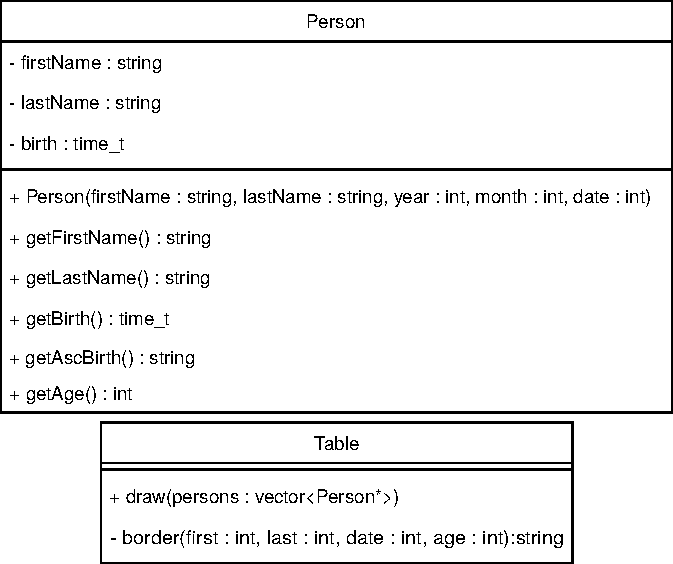
\includegraphics[scale=.6]{class_diagram.pdf}
    \end{center}
\end{frame}

\begin{frame}
    Hogyan működnek együtt az objektumok?
    \begin{center}
        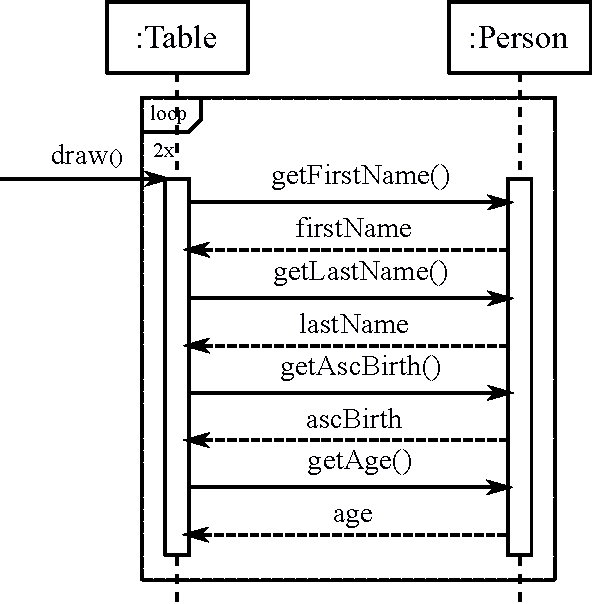
\includegraphics[scale=.6]{sequence_diagram.pdf}
    \end{center}
\end{frame}

\begin{frame}
    \begin{exampleblock}{\textattachfile{15/Person.h}{15/Person.h}}
        \small
        \lstinputlisting[style=cpp,linerange={8-17},numbers=left,firstnumber=8]{15/Person.h}
    \end{exampleblock}
\end{frame}
  
\begin{frame}
    \begin{exampleblock}{\textattachfile{15/Person.h}{15/Person.h}}
        \small
        \lstinputlisting[style=cpp,linerange={18-28},numbers=left,firstnumber=18]{15/Person.h}
    \end{exampleblock}
\end{frame}

\begin{frame}
    \begin{exampleblock}{\textattachfile{15/Person.cpp}{15/Person.cpp}}
        \small
        \lstinputlisting[style=cpp,linerange={11-18},numbers=left,firstnumber=11]{15/Person.cpp}
    \end{exampleblock}
\end{frame}

\begin{frame}
    \begin{exampleblock}{\textattachfile{15/Person.cpp}{15/Person.cpp}}
        \small
        \vspace{-0.3cm}
        \lstinputlisting[style=cpp,linerange={20-32},numbers=left,firstnumber=20]{15/Person.cpp}
        \vspace{-0.3cm}
    \end{exampleblock}
\end{frame}

\begin{frame}
    \begin{exampleblock}{\textattachfile{15/Table.h}{15/Table.h}}
        \lstinputlisting[style=cpp,linerange={10-15},numbers=left,firstnumber=10]{15/Table.h}
    \end{exampleblock}
\end{frame}

\begin{frame}
    \begin{exampleblock}{\textattachfile{15/Table.cpp}{15/Table.cpp}}
        \vspace{-0.3cm}
        \scriptsize
        \lstinputlisting[style=cpp,linerange={3-19},numbers=left,firstnumber=3]{15/Table.cpp}
        \vspace{-0.3cm}
    \end{exampleblock}
\end{frame}

\begin{frame}
    \begin{exampleblock}{\textattachfile{15/Table.cpp}{15/Table.cpp}}
        \footnotesize
        \lstinputlisting[style=cpp,linerange={20-29},numbers=left,firstnumber=20]{15/Table.cpp}
    \end{exampleblock}
\end{frame}

\begin{frame}
    \begin{exampleblock}{\textattachfile{15/Table.cpp}{15/Table.cpp}}
        \footnotesize
        \lstinputlisting[style=cpp,linerange={31-40},numbers=left,firstnumber=31]{15/Table.cpp}
    \end{exampleblock}
\end{frame}

\begin{frame}
    \begin{exampleblock}{\textattachfile{15/main.cpp}{15/main.cpp}}
        \small
        \lstinputlisting[style=cpp,linerange={5-17},numbers=left,firstnumber=5]{15/main.cpp}
    \end{exampleblock}
\end{frame}

\begin{frame}[fragile]
    \begin{block}{Kimenet \\ \texttt{g++ -std=c++11 -o main Person.cpp Table.cpp main.cpp \&\& ./main}}
        \begin{verbatim}
+---------------+-----------+-----+
|  Andras Arato |  9/3/1921 | 101 |
|    Bela Bokor | 2/12/1978 |  43 |
| Cecilia Cudar | 21/5/2013 |   9 |
+---------------+-----------+-----+
\end{verbatim}
    \end{block}
\end{frame}

\section{Mock-olás}

\begin{frame}
    Mock-olás előkészítése
    \begin{itemize}
        \item Mock osztály származtatása a \emph{hívott} osztályból (\texttt{MockPerson})
        \item Lehetőleg a virtuális függvényeit mock-oljuk (egyszerűbb)
        \item Legyen a destruktora is virtuális; a hívások számát az objektum törlésekor ellenőrzi a gMock
        \item A származtatott (mock) osztály \emph{nyilvános} részében jelöljük meg a mock-olandó függvényeket (\texttt{MOCK\_METHOD()})
        \item A makró paraméterei a visszatérési érték típusa, a függvény neve, paraméterlistája.
        \item Negyedikként állhat \texttt{const} a konstans függvényeknél, és \texttt{override} a virtuállis függvények felüldefiniálásánál.
    \end{itemize}
\end{frame}

\begin{frame}
    \begin{exampleblock}{\textattachfile{15/MockPerson.h}{15/MockPerson.h}}
        \footnotesize
        \lstinputlisting[style=cpp,numbers=left]{15/MockPerson.h}
    \end{exampleblock}
\end{frame}

\begin{frame}
    Teszt osztály előkészítése
    \begin{itemize}
        \item Tegyük ismertté (\texttt{using}) a gMock névterében lévő, felhasználandó azonosítókat (pl. \texttt{Return})!
        \item Hozzunk létre teszt eseteket a már ismert módon!
        \item Példányosítsuk a mock osztályt, majd definiáljuk az elvárásokat (\texttt{EXPECT\_CALL}).
        \item Csak ezután kezdeményezzük a hívásokat! (Különben definiálatlan működés.)
        \item Szabadítsuk fel az objektumokat!
    \end{itemize}
\end{frame}

\begin{frame}
    \begin{exampleblock}{\textattachfile{15/PersonTest.cpp}{15/PersonTest.cpp}}
        \footnotesize
        \lstinputlisting[style=cpp,numbers=left,linerange={1-14}]{15/PersonTest.cpp}
    \end{exampleblock}
\end{frame}

\begin{frame}
    \begin{exampleblock}{\textattachfile{15/PersonTest.cpp}{15/PersonTest.cpp}}
        \footnotesize
        \lstinputlisting[style=cpp,numbers=left,linerange={15-26},firstnumber=15]{15/PersonTest.cpp}
    \end{exampleblock}
\end{frame}

\begin{frame}{}
    Konfiguráljuk a \texttt{cmake}-et!
    \begin{exampleblock}{\textattachfile{15/CMakeLists.txt}{15/CMakeLists.txt}}
        \footnotesize
        \lstinputlisting[style=cpp,numbers=left,linerange={19-29},firstnumber=19]{15/CMakeLists.txt}
    \end{exampleblock}
\end{frame}

\begin{frame}[fragile]
    \texttt{cmake -S . -B build}\\
    \texttt{cmake -{-}build build}\\
    \texttt{cd build \&\& ./person\_mock}\\
    \begin{block}{Kimenet}
        \scriptsize
        \vspace{-.4cm}
        \begin{verbatim}
Running main() from /.../15/build/_deps/googletest-src/googletest/src/gtest_main.cc
[==========] Running 1 test from 1 test suite.
[----------] Global test environment set-up.
[----------] 1 test from PersonTest
[ RUN      ] PersonTest.getFirstName
+--------------+----------+-----+
| Andras Arato | 9/3/1921 | 101 |
+--------------+----------+-----+
[       OK ] PersonTest.getFirstName (0 ms)
[----------] 1 test from PersonTest (0 ms total)

[----------] Global test environment tear-down
[==========] 1 test from 1 test suite ran. (0 ms total)
[  PASSED  ] 1 test.
\end{verbatim}
        \vspace{-.4cm}
    \end{block}
\end{frame}

\begin{frame}[fragile]
    Hogyan értesülünk a hibákról?
    \begin{exampleblock}{\textattachfile{15/PersonTest_hiba1.cpp}{15/PersonTest\_hiba1.cpp}}
        \footnotesize
        \lstinputlisting[style=cpp,numbers=left,linerange={12-14},firstnumber=12]{15/PersonTest_hiba1.cpp}
    \end{exampleblock}
    \begin{block}{Kimenet}
        \vspace{-.4cm}
        \small
        \begin{verbatim}
Mock function called more times than expected - returning default value.
    Function call: getFirstName()
          Returns: ""
         Expected: to be called once
           Actual: called twice - over-saturated and active    
\end{verbatim}
        \vspace{-.4cm}
    \end{block}
\end{frame}

\begin{frame}[fragile]
    A mock objektum nem \emph{teszteli} a visszatérési értéket, hanem \emph{injektálja} azt! $\to$ Az ős osztály állhat akár csupa pure virtual függvényből.
    \begin{exampleblock}{\textattachfile{15/PersonTest_hiba2.cpp}{15/PersonTest\_hiba2.cpp}}
        \footnotesize
        \lstinputlisting[style=cpp,numbers=left,linerange={21-24},firstnumber=21]{15/PersonTest_hiba2.cpp}
    \end{exampleblock}
    \begin{block}{Kimenet}
        \vspace{-.4cm}
        \small
        \begin{verbatim}
Expected equality of these values:
  101
  andras->getAge()
    Which is: -1234    
\end{verbatim}
        \vspace{-.4cm}
    \end{block}
\end{frame}

\begin{frame}[fragile]
    \begin{exampleblock}{Elvárások megadásának általános formája}
        \footnotesize
        EXPECT\_CALL(\emph{mock\_objektum}, \emph{tagfüggvény(illesztők)})\\
        \qquad .Times(\emph{számosság})\\
        \qquad .WillOnce(\emph{tevékenység})\\
        \qquad .WillRepeatedly(\emph{tevékenység});\\
    \end{exampleblock}
    \begin{exampleblock}{Az elvárások könnyen olvashatóak:}
        \footnotesize
        EXPECT\_CALL(*andras, getAge())\\
        \qquad .Times(5)\\
        \qquad .WillOnce(99)\\
        \qquad .WillOnce(100)\\
        \qquad .WillRepeatedly(101);\\
    \end{exampleblock}
    \footnotesize
    Azaz azt várjuk, hogy $5\times$ hívják majd az \texttt{andras} címen lévő objektum \texttt{getAge()} tagfüggvényét, 
    ami először 99, aztán 100, majd minden további alkalommal a 101 értékkel tér vissza.
\end{frame}

\begin{frame}
    A hívott tagfüggvény paraméterének elvárt értéke
    \begin{itemize}
        \item \texttt{EXPECT\_CALL(*andras, setFirstName("Bela"));} $\to$ pontosan ezt a paramétert kell kapnia
        \item \texttt{EXPECT\_CALL(*andras, setFirstName(\_));} $\to$ nem érdekel, \emph{milyen értékű} paramétert kap
        \item \texttt{EXPECT\_CALL(*andras, setFirstName);} $\to$ nem érdekel, \emph{milyen értékű és hány darab} paramétert kap; 
        a felültöltött változatok közül vajon \hiv{\href{https://google.github.io/googletest/gmock\_cook\_book.html\#SelectOverload}{melyik hívását}} várjuk el?
    \end{itemize}
    Az \_ a használható \hiv{\href{https://google.github.io/googletest/reference/matchers.html\#wildcard}{\emph{illesztők}}} egyike. Néhány példa:
    \begin{description}[mm]
        \item[\texttt{Eq(\emph{érték})}] egyezés vizsgálat 
        \item[\texttt{Ge(\emph{érték})}] a paraméter nagyobb, vagy egyenlő mint az \emph{érték}
        \item[\texttt{IsTrue()}] a paraméter kifejezés értéke \emph{igaz}
    \end{description}
    Akár \hiv{\href{https://google.github.io/googletest/gmock\_cook\_book.html\#NewMatchers}{saját illesztők}} is készíthetők.
\end{frame}

\begin{frame}
    Hívások elvárt mennyiségének kifejezése
    \begin{description}[mm]
        \item[\texttt{Times(\emph{n})}] pontosan \emph{n} ismétlés
        \item[\texttt{Times(0)}] speciálisan: egyszer sem szabad hívni a tagfüggvényt
        \item[\texttt{Times(AtLeast(\emph{n}))}] legalább \emph{n} ismétlés; \hiv{\href{https://google.github.io/googletest/reference/mocking.html\#EXPECT\_CALL.Times}{további lehetőségek}}
    \end{description}
    Az elvárt hívási mennyiséget a \texttt{WillOnce()} és \texttt{WillRepeatedly()} hívások számából is kitalálhatja:
    \begin{itemize}
        \item ha egyetlen ilyen záradék sem fordul elő $\to$ \texttt{Times(1)}
        \item egymást követi \emph{n} \texttt{WillOnce()}, de nincs egyetlen \texttt{WillRepeatedly()} sem $\to$ \texttt{Times(\emph{n})}
        \item egymást követi \emph{n} \texttt{WillOnce()} és egyetlen \texttt{WillRepeatedly()} $\to$ \texttt{Times(AtLeast(\emph{n}))}
    \end{itemize}
\end{frame}

\begin{frame}
    Tevékenységek
    \begin{itemize}
        \item Ha nem mondunk mást (\texttt{Return()}), a mock fv. visszatérési értékének típusa beépített típus vagy mutató $\to$ \emph{alapértelmezett tevékenység}, 
        pl. \texttt{void} visszatér érték nélkül, \texttt{bool} mindig \texttt{false}-szal tér vissza, mások 0-val.\\
        C++11 és újabbak: ha van alapértelmezett konstruktor, akkor az általa előállított értéket szolgáltatják.
        \item Ha nincs alapértelmezett tevékenység, vagy nem megfelelő, felülírhatjuk azt (pl. \texttt{Return(-1234)})
        \item Mi történik, ha a hívások száma nagyobb, mint a megadott tevékenységek száma? $\to$ alapértelmezett tevékenység
        \item Hogyan lehet referenciát visszaadni? $\to$ \texttt{ReturnRef(\emph{változó})}
        \item \hiv{\href{https://google.github.io/googletest/gmock\_cook\_book.html\#using-actions}{További lehetőségek}}
    \end{itemize}
\end{frame}

\begin{frame}{}
    Minden \texttt{Return()}-be írt kifejezés egyszer lesz kiértékelve $\to$ mellékhatások elmaradnak!
    \begin{exampleblock}{Mindig 100-at ad vissza!}
        int n = 100;\\
        EXPECT\_CALL(*andras, getAge())\\
        \qquad .Times(4)\\
        \qquad .WillRepeatedly(Return(n++));\\
    \end{exampleblock}
    Ha szeretnénk mellékhatásokat, \hiv{\href{https://google.github.io/googletest/gmock\_cook\_book.html\#MockingSideEffects}{saját tevékenységet}} kell készíteni.
\end{frame}

\begin{frame}
    Elvárások illesztése fordított sorrendben (új szabály felülírja a régit)
    \begin{exampleblock}{Mi történik, ha az elvárások az alábbiak:}
        EXPECT\_CALL(*andras, setFirstName(\_));\\
        EXPECT\_CALL(*andras, setFirstName("Daniel"))\\
        \qquad .Times(2);
    \end{exampleblock}
    majd
    \begin{itemize}
        \item \texttt{setFirstName("Daniel")}-t 3$\times$ hívják? $\to$ hiba
        \item \texttt{setFirstName("Daniel")}-t 2$\times$, majd \texttt{setFirstName("Endre")}-t 1$\times$? $\to$ OK
    \end{itemize}
    Általános elvárások előre (pl. bármilyen paraméterrel, \texttt{Times(AnyNumber())} $\to$ \hiv{\href{https://google.github.io/googletest/gmock\_cook\_book.html\#uninteresting-vs-unexpected}{váratlan}} hívások kerülése), speciálisak hátulra!
\end{frame}

\begin{frame}
    \footnotesize
    Az elvárt hívások tetszőleges sorrendben megtörténhetnek.
    \begin{exampleblock}{Hívások pontos sorrendjének előírása}
        \scriptsize
        TEST(PersonTest, pontosSorrend) \{ \\
        \qquad \dots \\
        \qquad \{ \\
        \qquad\qquad InSequence sorrend; \\
        \smallskip
        \qquad\qquad EXPECT\_CALL(*andras, getFirstName()); \\
        \qquad\qquad EXPECT\_CALL(*andras, getLastName()); \\
        \qquad\qquad EXPECT\_CALL(*andras, getAscBirth()); \\
        \qquad\qquad EXPECT\_CALL(*andras, getAge()); \\
        \qquad \} \\
        \qquad t.draw(persons); \\
        \qquad \dots \\
        \} %
    \end{exampleblock}
    \begin{itemize}
        \item Az \texttt{InSequence} objektum neve nem érdekes; a konstruktora teszi a dolgát.
        \item \hiv{\href{https://google.github.io/googletest/gmock\_cook\_book.html\#PartialOrder}{Részlegesen rendezett}} hívási sorrend is megadható.
    \end{itemize}
\end{frame}

\begin{frame}
    \small
    \begin{exampleblock}{Ragadós (sticky) elvárások}
        \scriptsize
        for (int i = n; i > 0; i-{-}) \{ \\
        \qquad EXPECT\_CALL(*andras, getFirstName()) \\
        \qquad\qquad .WillOnce(Return("Andras" + to\_string(i))); \\
        \}
    \end{exampleblock}
    Az illeszkedő elvárások aktívak maradnak $\to$ "Andras5", "Andras4", \dots helyett a második hívás után hiba!
    \begin{exampleblock}{Megoldás}
        \scriptsize
        \{ \\ %
        \qquad InSequence sorrend; \\
        \smallskip
        \qquad for (int i = n; i > 0; i-{-}) \{ \\
        \qquad\qquad EXPECT\_CALL(*andras, getFirstName()) \\
        \qquad\qquad\qquad .WillOnce(Return("Andras" + to\_string(i))) \\
        \qquad\qquad\qquad .RetiresOnSaturation(); \\
        \qquad \} \\
        \} %
    \end{exampleblock}
\end{frame}

\begin{frame}
    Érdektelen hívások
    \begin{itemize}
        \item Ha nem érdekes, mi történik egy függvénnyel $\to$ nem mondunk róla semmit
        \item Ha meghívják $\to$ figyelmeztető üzenet, de nem hiba (Naggy, kb. zsémbes)
        \item A viselkedés \hiv{\href{https://google.github.io/googletest/gmock\_cook\_book.html\#NiceStrictNaggy}{megváltoztatható}}
    \end{itemize}
\end{frame}

\end{document}